%%%%%%%%%%%%%%%%%%%%%%%%%%%%%%%%%%%%%%%%%
% Short Sectioned Assignment LaTeX Template Version 1.0 (5/5/12)
% This template has been downloaded from: http://www.LaTeXTemplates.com
% Original author:  Frits Wenneker (http://www.howtotex.com)
% License: CC BY-NC-SA 3.0 (http://creativecommons.org/licenses/by-nc-sa/3.0/)
%%%%%%%%%%%%%%%%%%%%%%%%%%%%%%%%%%%%%%%%%

%----------------------------------------------------------------------------------------
%	PACKAGES AND OTHER DOCUMENT CONFIGURATIONS
%----------------------------------------------------------------------------------------

\documentclass[paper=a4, fontsize=11pt]{scrartcl} % A4 paper and 11pt font size

% ---- Entrada y salida de texto -----

\usepackage[T1]{fontenc} % Use 8-bit encoding that has 256 glyphs
\usepackage[utf8]{inputenc}
%\usepackage{fourier} % Use the Adobe Utopia font for the document - comment this line to return to the LaTeX default

% ---- Idioma --------

\usepackage[spanish, es-tabla]{babel} % Selecciona el español para palabras introducidas automáticamente, p.ej. "septiembre" en la fecha y especifica que se use la palabra Tabla en vez de Cuadro

% ---- Otros paquetes ----

\usepackage{url} % ,href} %para incluir URLs e hipervínculos dentro del texto (aunque hay que instalar href)
\usepackage{hyperref}
\hypersetup{
	colorlinks=true,
	linkcolor=black,
	urlcolor=black,
	citecolor=black,
}
\usepackage{amsmath,amsfonts,amsthm} % Math packages
%\usepackage{graphics,graphicx, floatrow} %para incluir imágenes y notas en las imágenes
\usepackage{graphics,graphicx, float} %para incluir imágenes y colocarlas

% Para hacer tablas comlejas
%\usepackage{multirow}
%\usepackage{threeparttable}

%\usepackage{sectsty} % Allows customizing section commands
%\allsectionsfont{\centering \normalfont\scshape} % Make all sections centered, the default font and small caps

\usepackage{fancyhdr} % Custom headers and footers
\pagestyle{fancyplain} % Makes all pages in the document conform to the custom headers and footers
\fancyhead{} % No page header - if you want one, create it in the same way as the footers below
\fancyfoot[L]{} % Empty left footer
\fancyfoot[C]{} % Empty center footer
\fancyfoot[R]{\thepage} % Page numbering for right footer
\renewcommand{\headrulewidth}{0pt} % Remove header underlines
\renewcommand{\footrulewidth}{0pt} % Remove footer underlines
\setlength{\headheight}{13.6pt} % Customize the height of the header

\numberwithin{equation}{section} % Number equations within sections (i.e. 1.1, 1.2, 2.1, 2.2 instead of 1, 2, 3, 4)
\numberwithin{figure}{section} % Number figures within sections (i.e. 1.1, 1.2, 2.1, 2.2 instead of 1, 2, 3, 4)
\numberwithin{table}{section} % Number tables within sections (i.e. 1.1, 1.2, 2.1, 2.2 instead of 1, 2, 3, 4)

\setlength\parindent{0pt} % Removes all indentation from paragraphs - comment this line for an assignment with lots of text

\newcommand{\horrule}[1]{\rule{\linewidth}{#1}} % Create horizontal rule command with 1 argument of height
\usepackage{booktabs}

\usepackage{listings}
\usepackage{color}
\usepackage{xcolor}
\lstdefinestyle{customc}{
	belowcaptionskip=1\baselineskip,
	breaklines=true,
	frame=L,
	xleftmargin=\parindent,
	language=C,
	showstringspaces=false,
	basicstyle=\footnotesize\ttfamily,
	keywordstyle=\bfseries\color{green!40!black},
	commentstyle=\itshape\color{purple!40!black},
	identifierstyle=\color{blue},
	stringstyle=\color{orange},
}

\lstset{escapechar=@,style=customc}
\usepackage{url}

\title{	
	\normalfont \normalsize
	\begin{figure}[htb]
		\centering
		
\includegraphics[width=0.3\textwidth]{./imagenes/1}
	\end{figure}
	\textsc{\textbf{Inteligencia del Negocio} \\ Grado en Ingeniería Informática \\ 
	Curso 2018-2019} \\ https://consigna.ugr.es/f/6Ri6jjdgQ9BA5XGz/P1-Ramirez-Garcia-Felix.zip \\[10pt] % Your university, school and/or department name(s)
	\begin{figure}[htb]
		\centering
		
\includegraphics[width=0.25\textwidth]{./imagenes/2}
	\end{figure}
	\horrule{0.5pt} \\[0.4cm] % Thin top horizontal rule
	\huge Memoria Práctica 1 : Grupo 1  \\
	\huge Análisis Predictivo Empresarial Mediante Clasificación.
	\\ % The assignment title
	\horrule{2pt} \\[0.5cm] % Thick bottom horizontal rule
}
\author{Félix Ramírez García  \\
\href{mailto:felixramirezgarcia@correo.ugr.es}{felixramirezgarcia@correo.ugr.es}} % Nombre y apellidos
\date{\normalsize\today} % Incluye la fecha actual

%----------------------------------------------------------------------------------------
% DOCUMENTO
%----------------------------------------------------------------------------------------

\begin{document}
	
	\maketitle % Muestra el Título
	
	\newpage %inserta un salto de página
	
	\tableofcontents % para generar el índice de contenidos
	
	\listoffigures % para generar índice de imágenes.
	
	\listoftables % para generar índice de tablas.
	
	\newpage
	
	%-----------------------------------------------------------------------
	%							Introducci´on
	%----------------------------------------------------------------------	
	\section[Introducción]{Introducción.}

	Esta práctica ha sido llevada a cabo para la asignatura Inteligencia del Negocio de la universidad de Granada, asignatura de 
	cuarto curso del Grado en Ingeniería Informática. En ella veremos el uso de algoritmos de aprendizaje supervisado de clasificación
	para realizar el análisis predictivo de los datos que se describen a continuación. \\
	
	El contenido de noticias en la red esta	creciendo continuamente . Esto hace necesario para cualquier
	medio de comunicación la predicción del impacto que tengan las noticias en la sociedad . Pudiendo analizar los artículos antes
	de su publicación se pueden optimizar sus características para que tengan una mayor popularidad. \\
	
	El conjunto de datos \cite{sci2s.ugr.es} se basa en 39.644 noticias con valores perdidos extraídas en 2015. 
	Cada noticia tiene las siguientes características: \\
	
	\vspace{1mm}
	
		1. n\_tokens\_title:               			\hfill Número de palabras en el título \\
		2. n\_tokens\_content:             			\hfill Número de palabras en el contenido \\
		3. n\_unique\_tokens:              			\hfill Tasa de palabras únicas en el contenido \\
		4. n\_non\_stop\_words:             		\hfill Velocidad de palabras sin parar en el contenido \\
		5. n\_non\_stop\_unique\_tokens:     		\hfill Ritmo de palabras únicas sin parar en el contento \\
		6. num\_hrefs:                    			\hfill Número de enlaces \\
		7. num\_self\_hrefs:               			\hfill Número de enlaces a otros artículos publicados \\
		8. num\_imgs:                     			\hfill Número de imágenes \\
		9. num\_videos:                   			\hfill Número de vídeos \\
		10. longitud\_media\_del\_token:         	\hfill Longitud media de las palabras en el contento \\
		11. num\_keywords:                 			\hfill Número de palabras clave en los metadatos \\
		12. data\_channel\_is\_lifestyle:    		\hfill ¿Es el canal de datos "Estilo de vida"? \\
		13. data\_channel\_is\_entertainment:		\hfill ¿Es el canal de datos 'Entretenimiento'? \\
		14. data\_channel\_is\_bus:          		\hfill ¿Es el canal de datos'Business'? \\
		15. data\_channel\_is\_socmed:       		\hfill ¿Es el canal de datos 'Social Media'? \\
		16. data\_channel\_is\_tech:				\hfill ¿Es el canal de datos 'Tech'? \\
		17. data\_channel\_is\_world:        		\hfill ¿Es el canal de datos 'Mundo'? \\
		18. kw\_min\_min\_min:						\hfill Palabra clave peor Min \\
		19. kw\_max\_min: 							\hfill Palabra clave peor Max  \\
		20. kw\_avg\_min: 							\hfill Palabra clave peor, promedio \\
		21. kw\_min\_max:                   		\hfill Mejor palabra clave (min. acciones) \\
		22. kw\_max\_max:                   		\hfill Mejor palabra clave (porcentaje máximo) \\
		23. kw\_avg\_max:                   		\hfill Mejor palabra clave (promedio de acciones) \\
		24. kw\_min\_avg:							\hfill Palabra clave media (min. acciones) \\
		25. kw\_max\_avg:							\hfill Palabra clave media (máx. acciones) \\
		26. kw\_avg\_avg\_avg:						\hfill Palabra clave media (acciones medias) \\
		27. auto-referencia\_compartimentos\_mínimos: \hfill Participación mín de los referenciados \\
		28. auto-referencia\_compartimentos\_max:     \hfill Porcentaje máx de referenciados \\
		29. self\_reference\_avg\_sharess:   			\hfill Promedio de acciones de artículos referenciados \\
		30. día-de-la-semana-es-lunes:            	\hfill ¿El artículo fue publicado un lunes? \\
		31. día-de-la-semana-es-el-día-de-la-semana:\hfill ¿El artículo fue publicado un martes? \\
		32. día\_de\_la\_semana\_es\_miércoles:          \hfill ¿El artículo fue publicado un miércoles? \\
		33. dia-de-la-semana-es-jueves:		 		\hfill ¿El articulo se publico un jueves? \\
		34. día-de-la-semana-es-viernes:            \hfill ¿El artículo fue publicado un viernes? \\
		35. día-de-la-semana-es-sábado:          	\hfill ¿El artículo se publicó un sábado? \\
		36. día-de-la-semana-es-domingo:            \hfill ¿El artículo se publicó un domingo? \\
		37. is\_fin de semana:                   	\hfill ¿El artículo fue publicado el fin de semana? \\
		38. LDA\_00:									\hfill Cercanía al tema LDA 0 \\
		39. LDA\_01:									\hfill Cercanía al tema 1 de LDA \\
		40. LDA\_02:									\hfill Cercanía al tema 2 de LDA \\
		41. LDA\_03:									\hfill Cercanía al tema 3 de LDA \\
		42. LDA\_04:									\hfill Cercanía al tema 4 de LDA \\
		43. global\_subjetividad:          			\hfill Subjetividad del texto \\
		44. global\_sentiment\_polarity:    			\hfill Polaridad del sentimiento del texto \\
		45. global\_rate\_positive\_words:   			\hfill Índice de palabras positivas en el contenido \\
		46. global\_rate\_negative\_words:   			\hfill Tasa de palabras negativas en el contenido \\
		47. rate\_positive\_words:          			\hfill Tasa de palabras positivas entre los no neutrales  \\
		48. rate\_negative\_words:          			\hfill Tasa de palabras negativas entre los no neutrales  \\
		49. avg\_positive\_polarity:         			\hfill Polaridad media de las palabras positivas \\
		50. min\_polaridad\_positiva:        			\hfill Polaridad mínima de las palabras positivas \\
		51. max\_polaridad\_positiva:        			\hfill Polaridad máxima de las palabras positivas \\
		52. avg\_negativo\_polaridad:        			\hfill Polaridad media de las palabras negativas \\
		53. min\_polaridad\_negativa:        			\hfill Polaridad mínima de las palabras negativas \\
		54. max\_polaridad\_negativa:       			\hfill Polaridad máxima de las palabras negativas \\
		55. title\_subjectivity:           			\hfill Subjetividad del título \\
		56. title\_sentiment\_polarity:     			\hfill Polaridad del título \\
		57. abs\_title\_subjetividad:       			\hfill Nivel de subjetividad absoluta \\
		58. abs\_title\_sentiment\_polarity:			\hfill Nivel de polaridad absoluta \\
		59. clase:									\hfill popular o no\_popular (target) \\		
		
	\vspace{1mm}
	
	Por lo que se conoce el numero de veces que la noticia ha sido compartida, 
	se puede valorar si la noticia es popular o no. En nuestro caso, fijaremos como umbral 3000
	veces, de modo que si la noticia se comparte en un número superior a ese umbral, la noticia es
	considerada popular. \\

	Principalmente en esta práctica debemos abordar el estudio de los distintos algoritmos de clasificación
	mediante un diseño experimental apropiado extrayendo conclusiones finales.
	Para ello debemos aplicar seis algoritmos de clasificación distintos, y a su vez, sobre algunos de ellos, realizar 
	las modificaciones que se consideren oportunas para estudiar los comportamientos de los mismos sobre el problema que se estudia. \\

	Toda la experimentación se ha realizado sobre validación cruzada de 5 particiones. También se han extraído tablas comparativas para mostrar
	las diferencias de los algoritmos, gráficas ROC , matrices de confusión , G-mean , etc ...

	
	%-----------------------------------------------------------------------
	%							Resultados obtenidos
	%----------------------------------------------------------------------
	\section[Resultados obtenidos]{Resultados obtenidos.}

	Esta sección incluye un un apartado por cada uno de los seis algoritmos utilizados. 
	Para una primera toma de contacto , estos algoritmos han sido ejecutados con las opciones por defecto.
	Así como se han filtrado algunas columnas y se han rellenado valores perdidos con parámetros que han sido seleccionados 
	con aleatoriedad (Como la media) ,sin ningún estudio previo de los datos. \\

	El flujo de trabajo de todos los algoritmos comienza en el nodo lector del fichero , donde se cargan los datos. La 
	imagen 2.1 muestra el Workflow utilizado en KNIME para la ejecución y visualización del resultado de los algoritmos que detallamos en las siguientes subsecciones :

	\begin{figure}[htb]
		\centering
		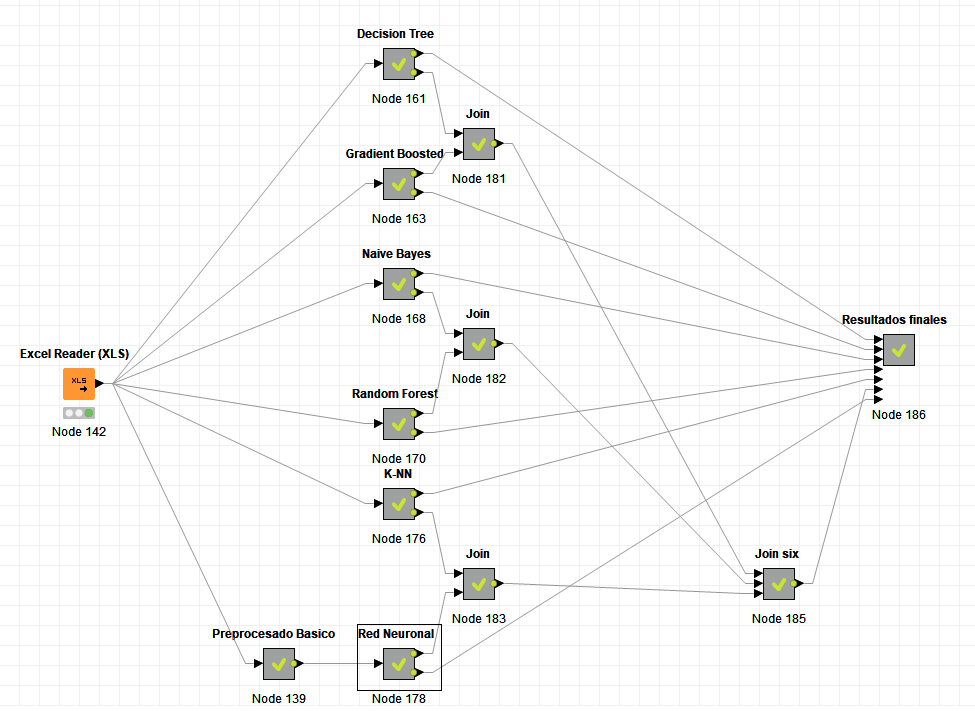
\includegraphics[width=0.9\textwidth]{./imagenes/33}
		\caption{Workflow en KNIME} \label{fig:33}
	\end{figure}

	%-----------------------------------------------------------------------
	%							Decision Tree
	%-----------------------------------------------------------------------

	\subsection{Decision Tree}

	En primer lugar usaremos el algoritmo de clasificación Decision Tree (Árbol de decisión) \cite{Wikipedia2} , el cual a partir 
	de un conjunto de datos permite determinar a que clase pertenece el caso de estudio. La 
	figura 2.2 muestra el Workflow utilizado en KNIME :
	
	\begin{figure}[htb]
		\centering
		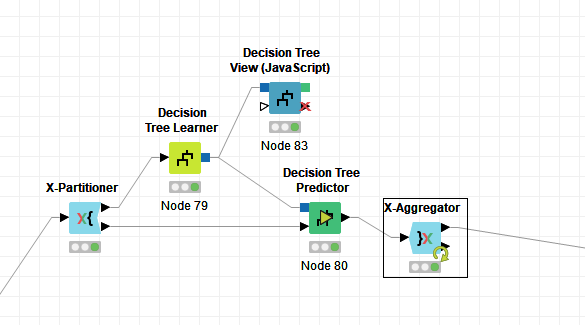
\includegraphics[width=0.5\textwidth]{./imagenes/6}
		\caption{Workflow del algoritmo Decision Tree} \label{fig:35}
	\end{figure}
	

	Dentro de los nodos usados para el algoritmo tenemos X-partitioner , que básicamente nos permite configurar el numero de validaciones
	(5 en nuestro caso) y el muestreo estratificado. Después tenemos los nodos del algoritmo , en primer lugar el Decision Tree Learner (nodo encargado del entrenamiento)
	, el cuál se encarga de recoger los datos de entrenamiento e inducir a partir de ellos un árbol de decisión, y en segundo lugar tenemos el nodo Decision Tree Predictor , el cual
	una vez obtenido un árbol de decisión se lo pasamos por el puerto de color azul, y por el otro puerto le pasamos el conjunto de datos de test , para así predecir
	el valor de la clase de nuevas muestras. Luego tenemos el nodo X-agregator  , que se encarga de volver a reproducir los nodos anteriores como si un bucle se tratara,
	y también se encarga de sacar una tabla con las particiones y la tabla de errores. Por ultimo usamos el nodo Scorer , que nos permite mostrar la matriz de confusión y las estadísticas del algoritmo. \\

	Para la obtención de los resultados de cada algoritmo se ha realizado en KNIME el Workflow que se muestra en la figura 2.3 ,y ya que se ha realizado el mismo flujo de trabajo para todos los algoritmos
	solo se va a exponer en esta subsección. En primer lugar nos encontramos con el nodo Scorer , que nos permite mostrar la matriz de confusión y las estadísticas del algoritmo. Los nodos posteriores
	tienen la función de filtrar estos datos y cambiar el identificador de la clase a predecir por el nombre del algoritmo que se este utilizando, de tal forma que podamos identificar los 
	resultados obtenidos por cualquier algoritmo. \\
	
	\begin{figure}[htb]
		\centering
		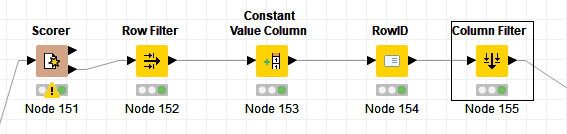
\includegraphics[width=0.5\textwidth]{./imagenes/35}
		\caption{Workflow para obtener los resultados de cada algoritmo} \label{fig:35}
	\end{figure}

	A continuación se muestran el siguiente contenido obtenido por Decision Tree :	\\
	Una tabla con la matriz de confusión. (Tabla 2.1) \\
	Una imagen con la tabla de errores .(Figura 2.4) \\
	Una imagen para la curva ROC. (Figura 2.5)	\\
	Una tabla con los datos resultantes de la ejecución del algoritmo (Tabla 2.2)\\

	\begin{table}[htbp]
		\begin{center}
			\begin{tabular}{ | c | c | c | }
				\hline
				x & Popular & NoPopular \\ \hline
				Popular & 2465 & 6456 \\ \hline 
				Nopopular & 5261 & 25450 \\ \hline
			  \end{tabular}
			\caption{Matriz de confisión de Decision Tree}
			\label{tabla:sencilla}
		\end{center}
	\end{table}

	\begin{figure}[htb]
		\centering
		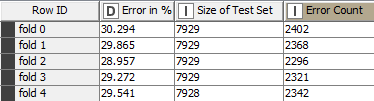
\includegraphics[width=0.6\textwidth]{./imagenes/8}
		\caption{Errores de Decision Tree} \label{fig:1}
	\end{figure}

	\begin{figure}[htb]
		\centering
		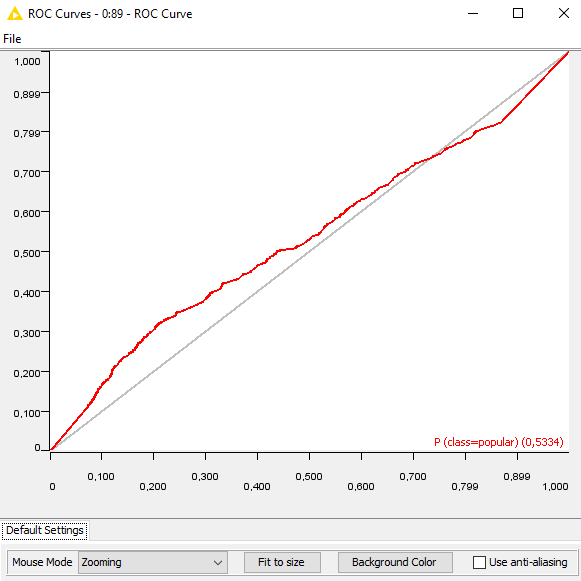
\includegraphics[width=0.4\textwidth]{./imagenes/9}
		\caption{Curva ROC de Decision Tree} \label{fig:1}
	\end{figure}

	\begin{table}[htbp]
		\begin{center}
			\begin{tabular}{|c|c|}
				\hline
				Medida & Valor \\
				\hline \hline
				Accuracy & 0,704 \\
				\hline
				TPR &  0,276 \\
				\hline
				FPR &  0,171 \\
				\hline
				TNR &  0,829 \\
				\hline
				FNR &  0,723 \\
				\hline
				AUC &  0,548 \\
				\hline
				F1-Score & 0,296 \\
				\hline	
				G-Mean & 0,479 \\
				\hline
			\end{tabular}
			\caption{Resultados de Decision Tree}
			\label{tabla:sencilla}
		\end{center}
	\end{table}

	%-----------------------------------------------------------------------
	%							Gradient Boosted
	%----------------------------------------------------------------------

	\subsection{Gradient Boosted}

	El segundo algoritmo que aplicamos es Gradient Boosted \cite{Wikipedia3} , el cual utiliza árboles 
	de regresión para construir un conjunto de árboles. El Workflow del algoritmo Gradient Boosted usado en KNIME 
	es el que muestra la figura 2.6 . \\

	\begin{figure}[htb]
		\centering
		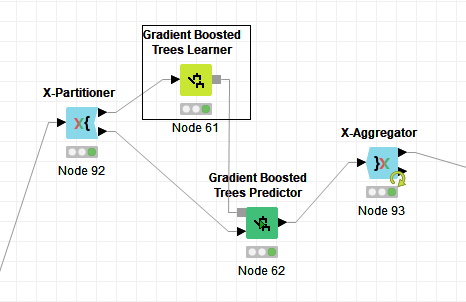
\includegraphics[width=0.6\textwidth]{./imagenes/10}
		\caption{Workflow del algoritmo Gradient Boosted} \label{fig:10}
	\end{figure}

	Dentro de los nodos usados para el algoritmo tenemos X-partitioner , que básicamente nos permite configurar el numero de validaciones
	(5 en nuestro caso) y el muestreo estratificado. Después tenemos los nodos del algoritmo , en primer lugar el Gradient Boosted Trees Learner (nodo encargado del entrenamiento)
	, y en segundo lugar tenemos el nodo Decision Gradient Boosted Trees Predictor , el cual clasifica los datos usando un modelo de Gradient Boosted Trees , para así predecir
	el valor de la clase de nuevas muestras. Luego tenemos el nodo X-agregator  , que se encarga de volver a reproducir los nodos anteriores como si un bucle se tratara,
	y también se encarga de sacar una tabla con las particiones y la tabla de errores. Por ultimo usamos el nodo Scorer , que nos permite mostrar la matriz de confusión y las estadísticas del algoritmo. \\

	A continuación se muestra el siguiente contenido obtenido por Gradient Boosted Decision Tree :	\\
	Una tabla con la matriz de confusión. (Tabla 2.3) \\
	Una imagen con la tabla de errores. (Figura 2.7) \\
	Una imagen para la curva ROC. (Figura 2.8)	\\
	Una tabla con los datos resultantes de la ejecución del algoritmo (Tabla 2.4)\\

	\begin{table}[htbp]
		\begin{center}
			\begin{tabular}{ | c | c | c | }
				\hline
				x & Popular & NoPopular \\ \hline
				Popular & 865 & 8061 \\ \hline 
				Nopopular & 697 & 30021 \\ \hline
			  \end{tabular}
			\caption{Matriz de confisión de Gradient Boosted Decision Tree}
			\label{tabla:sencilla}
		\end{center}
	\end{table}

	\begin{figure}[htb]
		\centering
		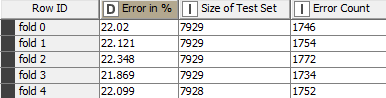
\includegraphics[width=0.6\textwidth]{./imagenes/11}
		\caption{Errores de Gradient Boosted Decision Tree} \label{fig:2}
	\end{figure}

	\begin{figure}[htb]
		\centering
		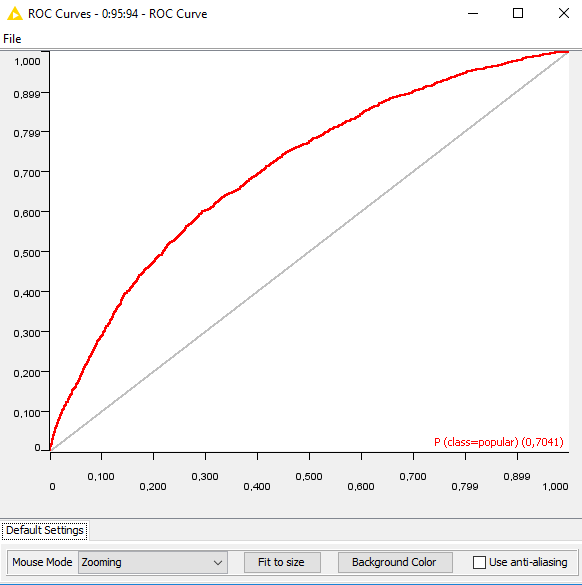
\includegraphics[width=0.4\textwidth]{./imagenes/12}
		\caption{Curva ROC de Gradient Boosted Decision Tree} \label{fig:1}
	\end{figure}

	\begin{table}[htbp]
		\begin{center}
			\begin{tabular}{|c|c|}
				\hline
				Medida & Valor \\
				\hline \hline
				Accuracy & 0,779 \\
				\hline
				TPR &  0,097 \\
				\hline
				FPR &  0,022 \\
				\hline
				TNR &  0,97 \\
				\hline
				FNR &  0,903 \\
				\hline
				AUC &  0,715 \\
				\hline
				F1-Score & 0,165 \\
				\hline	
				G-Mean & 0,308 \\
				\hline
			\end{tabular}
			\caption{Resultados de Gradient Boosted Decision Tree}
			\label{tabla:sencilla}
		\end{center}
	\end{table}

	%-----------------------------------------------------------------------
	%							Random Forest
	%----------------------------------------------------------------------

	\subsection{Random Forest}

	El tercer algoritmo que usaremos será Random Forest \cite{Wikipedia4} , el cuál es una
	combinación de arboles predictivos tal que cada árbol depende de los valores de un vector aleatorio
	 probado independientemente y con la misma distribución para cada uno de estos.

	El Workflow del algoritmo Random Forest usado en KNIME 
	es el que muestra la figura 2.9 . 

	\begin{figure}[htb]
		\centering
		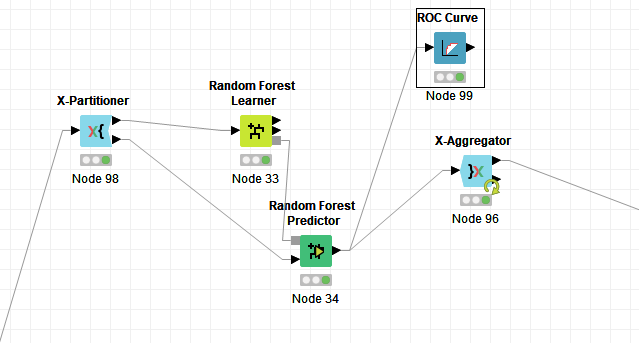
\includegraphics[width=0.6\textwidth]{./imagenes/13}
		\caption{Workflow del algoritmo Random Forest} \label{fig:13}
	\end{figure}

	Dentro de los nodos usados para el algoritmo tenemos X-partitioner , que básicamente nos permite configurar el numero de validaciones
	(5 en nuestro caso) y el muestreo estratificado. Después tenemos los nodos del algoritmo , en primer lugar el Random Forest Learner (nodo encargado del entrenamiento)
	, y en segundo lugar tenemos el nodo Random Forest Predictor , el cual predice patrones de acuerdo a los árboles
	individuales en un modelo de bosque aleatorio. Luego tenemos el nodo X-agregator  , que se encarga de volver a reproducir los nodos anteriores como si un bucle se tratara,
	y también se encarga de sacar una tabla con las particiones y la tabla de errores. Por ultimo usamos el nodo Scorer , que nos permite mostrar la matriz de confusión y las estadísticas del algoritmo. \\

	A continuación se muestra el siguiente contenido obtenido por Random Forest :	\\
	Una imagen con la matriz de confusión. (Figura 2.10) \\
	Una imagen con la tabla de errores. (Figura 2.11) \\
	Una imagen para la curva ROC. (Figura 2.12)	\\
	Una tabla con los datos resultantes de la ejecución del algoritmo (Tabla 2.5)\\

	\begin{figure}[htb]
		\centering
		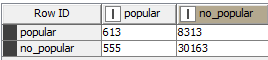
\includegraphics[width=0.5\textwidth]{./imagenes/14}
		\caption{Matriz de confisión de Random Forest} \label{fig:2}
	\end{figure}

	\begin{figure}[htb]
		\centering
		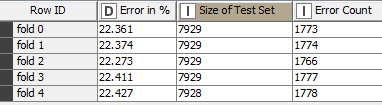
\includegraphics[width=0.6\textwidth]{./imagenes/15}
		\caption{Errores de Random Forest} \label{fig:2}
	\end{figure}

	\begin{figure}[htb]
		\centering
		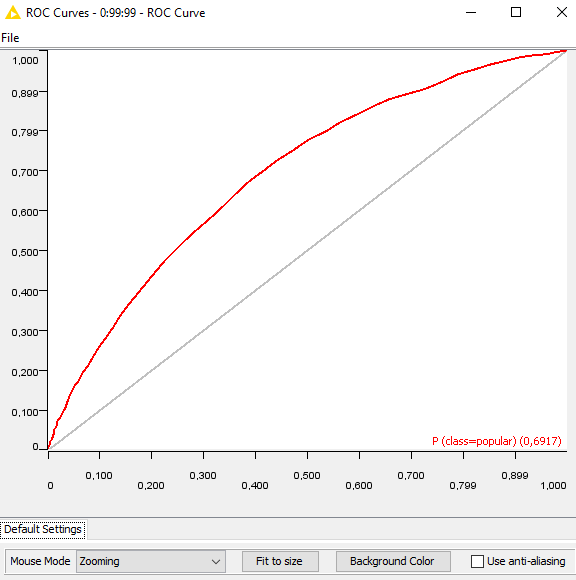
\includegraphics[width=0.4\textwidth]{./imagenes/16}
		\caption{Curva ROC de Random Forest} \label{fig:1}
	\end{figure}

	\begin{table}[htbp]
		\begin{center}
			\begin{tabular}{|c|c|}
				\hline
				Medida & Valor \\
				\hline \hline
				Accuracy & 0,776 \\
				\hline
				TPR &  0,069 \\
				\hline
				FPR &  0,018 \\
				\hline
				TNR &  0,982 \\
				\hline
				FNR &  0,93 \\
				\hline
				AUC &  0,7 \\
				\hline
				F1-Score & 0,121 \\
				\hline	
				G-Mean & 0,259 \\
				\hline
			\end{tabular}
			\caption{Resultados de Random Forest}
			\label{tabla:sencilla}
		\end{center}
	\end{table}

	%-----------------------------------------------------------------------
	%							Naive Bayes
	%----------------------------------------------------------------------

	\subsection{Naive Bayes}

	El cuarto algoritmo que usaremos es un clasificador de Bayes \cite{Wikipedia1}, éste asume que la presencia o ausencia de una característica
	particular no está relacionada con la presencia o ausencia de cualquier otra característica, dada la clase variable.
	
	\vspace{1mm}

	Un clasificador de Bayes considera que cada una de estas características contribuye de manera independiente a la probabilidad 
	de que una noticia sea popular, independientemente de la presencia o ausencia de las otras características.
	El flujo de trabajo empleado en KNIME es el que se muestra en la figura 2.13

	\begin{figure}[htb]
		\centering
		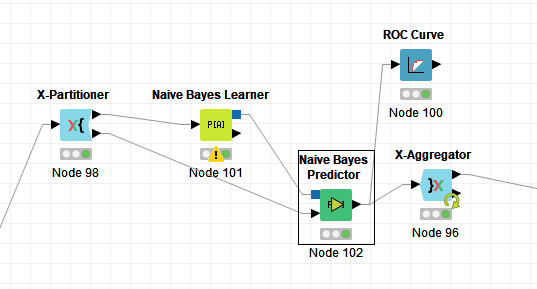
\includegraphics[width=0.6\textwidth]{./imagenes/18}
		\caption{Workflow del algoritmo Naive Bayes} \label{fig:1}
	\end{figure}

	Dentro de los nodos usados para el algoritmo tenemos X-partitioner , que básicamente nos permite configurar el numero de validaciones
	(5 en nuestro caso) y el muestreo estratificado. Después tenemos los nodos del algoritmo , en primer lugar el Naive Bayes Learner (nodo encargado del entrenamiento)
	el cual crea un modelo bayesiano, y en segundo lugar tenemos el nodo Naive Bayes Predictor , el cual predice la clase asociada
	según el modelo aprendido . Luego tenemos el nodo X-agregator  , que se encarga de volver a reproducir los nodos anteriores como si un bucle se tratara,
	y también se encarga de sacar una tabla con las particiones y la tabla de errores. Por ultimo usamos el nodo Scorer , que nos permite mostrar la matriz de confusión y las estadísticas del algoritmo. \\

	A continuación se muestra el siguiente contenido obtenido por Naive Bayes:	\\
	Una imagen con la matriz de confusión. (Figura 2.14) \\
	Una imagen con la tabla de errores. (Figura 2.15) \\
	Una imagen para la curva ROC. (Figura 2.16)	\\
	Una tabla con los datos resultantes de la ejecución del algoritmo (Tabla 2.6)\\

	\begin{figure}[htb]
		\centering
		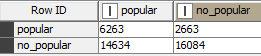
\includegraphics[width=0.5\textwidth]{./imagenes/19}
		\caption{Matriz de confisión de Naive Bayes} \label{fig:2}
	\end{figure}

	\begin{figure}[htb]
		\centering
		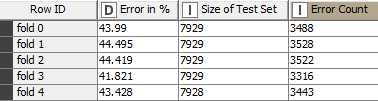
\includegraphics[width=0.6\textwidth]{./imagenes/20}
		\caption{Errores de Naive Bayes} \label{fig:2}
	\end{figure}

	\begin{figure}[htb]
		\centering
		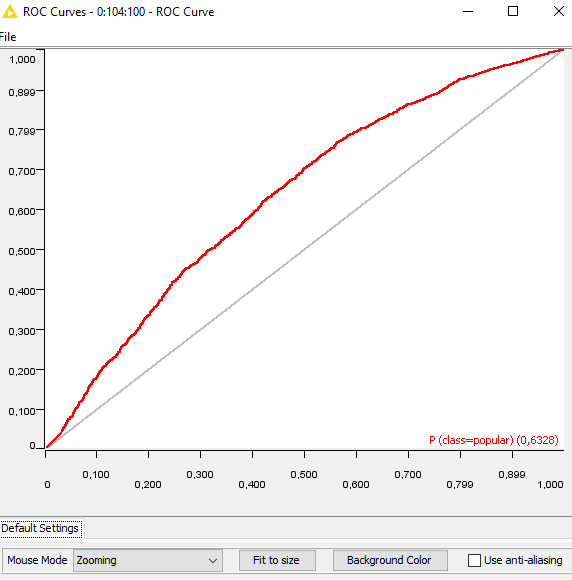
\includegraphics[width=0.4\textwidth]{./imagenes/21}
		\caption{Curva ROC de Naive Bayes} \label{fig:1}
	\end{figure}

	\begin{table}[htbp]
		\begin{center}
			\begin{tabular}{|c|c|}
				\hline
				Medida & Valor \\
				\hline \hline
				Accuracy & 0,564 \\
				\hline
				TPR &  0,702 \\
				\hline
				FPR &  0,018 \\
				\hline
				TNR &  0,524 \\
				\hline
				FNR &  0,93 \\
				\hline
				AUC &  0,645 \\
				\hline
				F1-Score & 0,42 \\
				\hline	
				G-Mean & 0,606 \\
				\hline
			\end{tabular}
			\caption{Resultados de Naive Bayes}
			\label{tabla:sencilla}
		\end{center}
	\end{table}

	%-----------------------------------------------------------------------
	%							K-NN
	%----------------------------------------------------------------------

	\subsection{K-NN}

	El quinto algoritmo clasificador que usaremos es el de los N vecinos mas cercanos k-NN  \cite{Wikipedia5} . Básicamente calcula las distancias 
	con todos los miembros de la colección y se toma un número K que son los que tienen la menor distancia. La mejor elección de k 
	depende fundamentalmente de los datos y generalmente, valores grandes de k reducen el efecto de ruido en la clasificación, pero crean límites entre clases parecidas. \\

	El flujo de trabajo empleado en KNIME es el que se muestra en la figura 2.17

	\begin{figure}[htb]
		\centering
		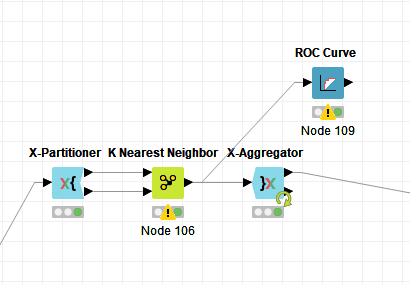
\includegraphics[width=0.5\textwidth]{./imagenes/22}
		\caption{Workflow del algoritmo K-NN} \label{fig:1}
	\end{figure}

	Dentro de los nodos usados para el algoritmo tenemos X-partitioner , que basicamente nos permite configurar el numero de validaciones
	(5 en nuestro caso) y el muestreo estratificado. Después tenemos el nodo del algoritmo , nodo con dos entradas , una para el aprendizaje y otra para los test , y una única salida.
	La parte de pre-procesado es necesaria para obtener un buen modelo tras el funcionamiento del algoritmo , ya que ignora los registros que tienen valores perdidos y las variables numéricas
	tienen que estar normalizadas. Pero para esta primera ejecución no se ha realizado el pre-procesado, éste se realizara en las secciones posteriores. Luego tenemos el nodo X-agregator  , que se encarga de volver a reproducir los nodos anteriores como si un bucle se tratara,
	y cambien se encarga de sacar una tabla con las particiones y la tabla de errores. Por ultimo usamos el nodo Scorer , que nos permite mostrar la matriz de confusión y las estadísticas del algoritmo. \\

	A continuación se muestra el siguiente contenido obtenido por K-NN:	\\
	Una imagen con la matriz de confusión. (Figura 2.18) \\
	Una imagen con la tabla de errores. (Figura 2.19) \\
	Una imagen para la curva ROC. (Figura 2.20)	\\
	Una tabla con los datos resultantes de la ejecución del algoritmo (Tabla 2.7)\\

	\begin{figure}[htb]
		\centering
		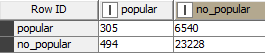
\includegraphics[width=0.5\textwidth]{./imagenes/23}
		\caption{Matriz de confisión de K-NN} \label{fig:2}
	\end{figure}

	\begin{figure}[htb]
		\centering
		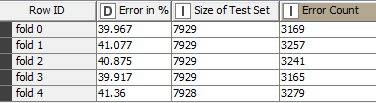
\includegraphics[width=0.6\textwidth]{./imagenes/24}
		\caption{Errores de K-NN} \label{fig:2}
	\end{figure}

	\begin{figure}[htb]
		\centering
		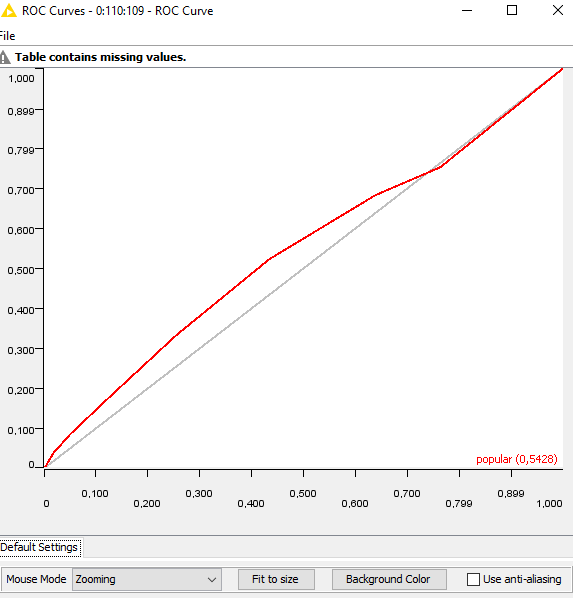
\includegraphics[width=0.4\textwidth]{./imagenes/25}
		\caption{Curva ROC de K-NN} \label{fig:1}
	\end{figure}

	\begin{table}[htbp]
		\begin{center}
			\begin{tabular}{|c|c|}
				\hline
				Medida & Valor \\
				\hline \hline
				Accuracy & 0,77 \\
				\hline
				TPR &  0,045 \\
				\hline
				FPR &  0,016 \\
				\hline
				TNR &  0,979 \\
				\hline
				FNR &  0,955 \\
				\hline
				AUC &  0,554 \\
				\hline
				F1-Score & 0,798 \\
				\hline	
				G-Mean & 0,209 \\
				\hline
			\end{tabular}
			\caption{Resultados de K-NN}
			\label{tabla:sencilla}
		\end{center}
	\end{table}

	%----------------------------------------------------------------------
	%							Red Neuronal
	%----------------------------------------------------------------------

	\subsection{Red Neuronal}

	El sexto algoritmo que usamos es el de Red Neuronal \cite{Wikipedia6} , un modelo computacional basado en un gran conjunto de unidades 
	neuronales simples. Cada neurona está conectada a otras , pudiendo incrementar los enlaces entre ellas el estado de activación de las adyacentes. \\
	
	Al igual que para el caso de de K-NN , para poder ejecutar el algoritmo se requiere que las columnas categóricas con datos de tipo string sean transformadas a columnas numéricas , y que 
	sean tratados los valores perdidos.  \\

	El flujo de trabajo empleado en KNIME es el que se muestra en las figuras 2.21 y 2.22. \\
	
	La figura 2.21 muestra el contenido del metanodo del pre-procesado , que consiste en un nodo para rellenar los valores perdidos , otro para filtrar la columna que es un string , y otro 
	nodo para normalizar los valores numéricos. 

	\begin{figure}[htb]
		\centering
		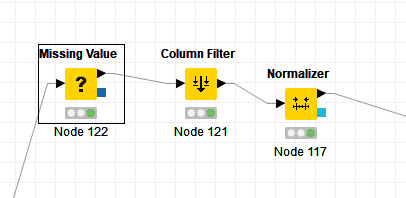
\includegraphics[width=0.5\textwidth]{./imagenes/26}
		\caption{Workflow del preprocesado para la Red Neuronal} \label{fig:1}
	\end{figure}
	
	La figura 2.22 muestra el contenido del algoritmo de Red Neuronal. Aparte de los nodos para realizar la validación cruzada , tenemos el nodo Rprop MLP Learner , que implementa el 
	algoritmo Rprop para redes feedforward multicapa. A la derecha de este nodo tenemos el nodo MultiLayer Perception Predictor, que en base a el modelo proporcionado , calcula los valores de salida.


	\begin{figure}[htb]
		\centering
		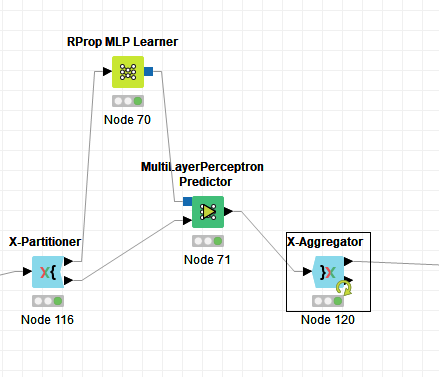
\includegraphics[width=0.5\textwidth]{./imagenes/27}
		\caption{Workflow del algoritmo de Red Neuronal} \label{fig:1}
	\end{figure}

	A continuación se muestra el siguiente contenido obtenido por Red Neuronal:	\\
	Una imagen con la matriz de confusión. (Figura 2.23) \\
	Una imagen con la tabla de errores. (Figura 2.24) \\
	Una imagen para la curva ROC. (Figura 2.25)	\\
	Una tabla con los datos resultantes de la ejecución del algoritmo (Tabla 2.8)\\

	\begin{figure}[htb]
		\centering
		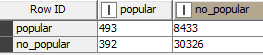
\includegraphics[width=0.4\textwidth]{./imagenes/29}
		\caption{Matriz de confisión de Red Neuronal} \label{fig:2}
	\end{figure}

	\begin{figure}[htb]
		\centering
		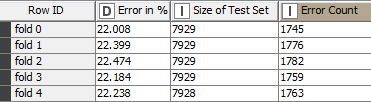
\includegraphics[width=0.6\textwidth]{./imagenes/28}
		\caption{Errores de Red Neuronal} \label{fig:2}
	\end{figure}

	\begin{figure}[htb]
		\centering
		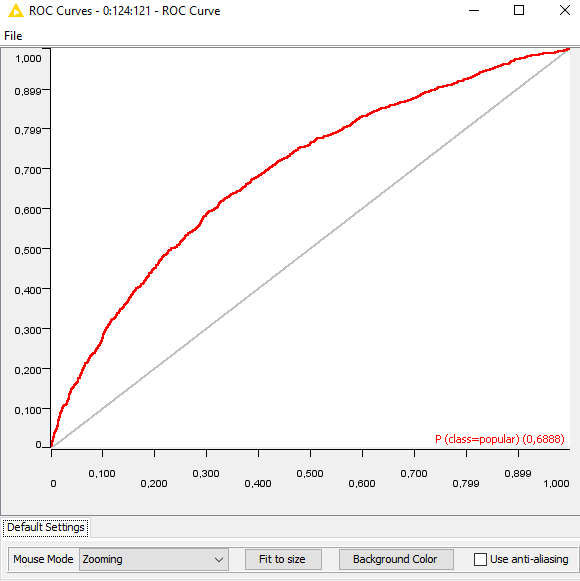
\includegraphics[width=0.4\textwidth]{./imagenes/30}
		\caption{Curva ROC de Red Neuronal} \label{fig:1}
	\end{figure}

	\begin{table}[htbp]
		\begin{center}
			\begin{tabular}{|c|c|}
				\hline
				Medida & Valor \\
				\hline \hline
				Accuracy & 0,777 \\
				\hline
				TPR &  0,055 \\
				\hline
				FPR &  0,012 \\
				\hline
				TNR &  0,987 \\
				\hline
				FNR &  0,945 \\
				\hline
				AUC &  0,695 \\
				\hline
				F1-Score & 0,1 \\
				\hline	
				G-Mean & 0,223 \\
				\hline
			\end{tabular}
			\caption{Resultados de Red Neuronal}
			\label{tabla:sencilla}
		\end{center}
	\end{table}
	
	%----------------------------------------------------------------------
	%							An´alisis de resultados
	%----------------------------------------------------------------------	
	\section[Análisis de resultados]{Análisis de resultados.}
	
	En este apartado se va a proceder al análisis comparativo de los distintos algoritmos teniendo en cuenta la tabla final de resultados, 
	la gráfica ROC , y las distintas gráficas dispuestas para en análisis. Para poder realizar el análisis se han obtenido los resultados de cada algoritmo ,
	y estos se han ido uniendo dos a dos con diferentes nodos Joiner para 
	poder crear un metanodo que contenga los resultados de todos. El contenido del metanodo es el que se muestra en la figura 3.1 , y partimos desde este punto para la generación de visualizaciones. 	\\

	\begin{figure}[htb]
		\centering
		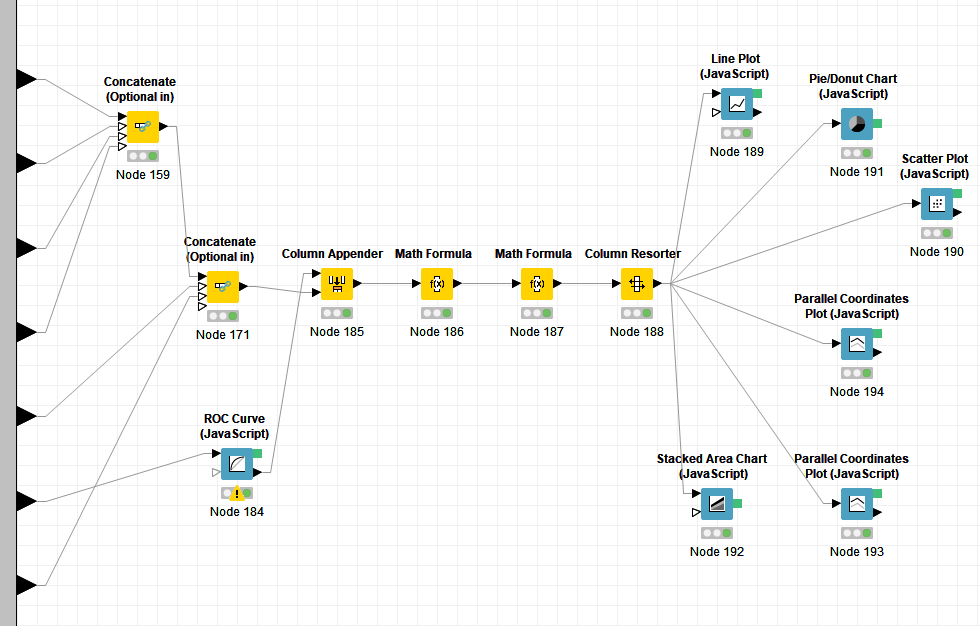
\includegraphics[width=0.8\textwidth]{./imagenes/36}
		\caption{Metanodo para la generacion de visualizaciones} \label{fig:1}
	\end{figure}

	En primer lugar tenemos la Figura final de resultados de todos los algoritmos juntos . La Figura 3.2

	\begin{figure}[htb]
		\centering
		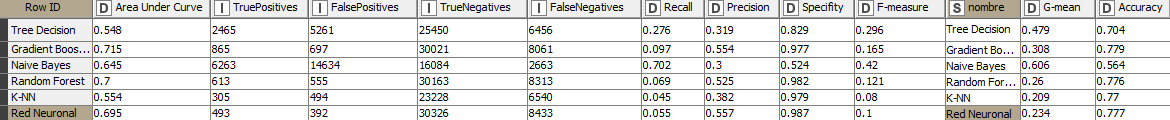
\includegraphics[width=1.0\textwidth]{./imagenes/34}
		\caption{Resultados de los diferentes algoritmos} \label{fig:1}
	\end{figure}

	Y en segundo lugar tenemos la imagen de la comparativa entre las distintas curvas ROC. 

	\begin{figure}[htb]
		\centering
		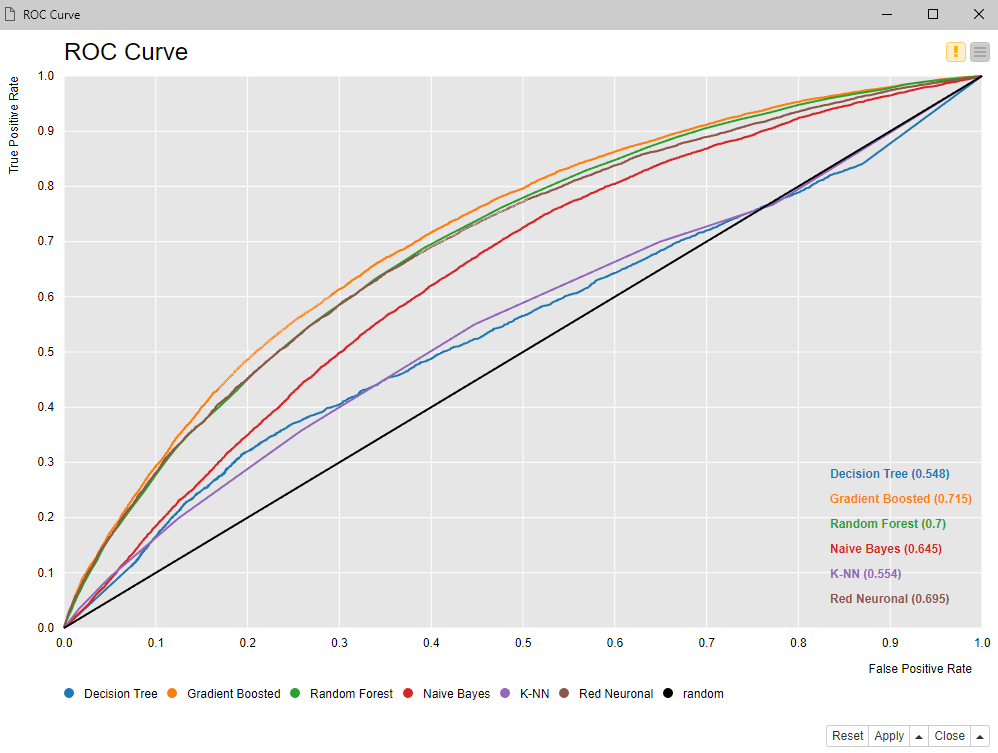
\includegraphics[width=0.8\textwidth]{./imagenes/32}
		\caption{Curvas ROC de los diferentes algoritmos} \label{fig:1}
	\end{figure}

	A partir de la tabla de resultados y de la gráfica ROC se pueden intuir varias cosas, la primera y más importante 
	es que los algoritmos que mejores resultados obtuvieron son el GradientBoosted , el RandomForest y el de Red Neuronal, 
	un poco peor se encuentra el NaiveBayes y los dos que obtuvieron peores resultados fueron el DecisionTree y el K-NN. \\

	La existencia de la diferencia entre los tres mejores y el Decision Tree es esperada, ya que estos tres primeros son 
	bastante mas completos. Mas completos desde el punto de vista de que por ejemplo Gradient Boosted crea diferentes arboles
	de los cuales va corrigiendo errores conforme va aprendiendo de los anteriores, permitiendo crear un modelo mas estable 
	que un solo árbol de decisión. También algo que les beneficia a GradientBoosted y a RandomForest es que son menos propensos 
	al sobre-ajuste en en entrenamiento.  \\

	El algoritmo de Red Neuronal es ideal para problemas complejos, pero con el se obtiene un modelo de caja negra , tiene mayor carga computacional
	y es propenso al sobre-ajuste. En este primer caso se ha obtenido un modelo bastante bueno , estando a la par con RandomForest. \\

	Por lo que respecta al pesimo resultado de K-NN , se puede deber a su configuración por defecto , ya que al tener en cuenta solamente a los 3 vecinos mas cercanos
	comenzaría su ejecución estando más penalizado que los demás algoritmos. \\

	En cuanto a los resultados obtenidos de los seis algoritmos respecto al Recall o TPR se tiene la figura 3.4. En ella se tienen en cuenta las variables
	de verdaderos positivos y falsos negativos, que son las que intervienen en el calculo del Recall. En esta gráfica se puede apreciar porque unos algoritmos tienen 
	mejor Recall que otros. En primer lugar empezamos con el algoritmo Naive Bayes , el que mejor Recall tiene, tiene muchos verdaderos positivos y pocos falsos negativos. 
	A este algoritmo le sigue el de Decision Tree , pero con unos valores bastante inferiores. Por ultimo tenemos a los demás algoritmos , que tienen unos valores pésimos muy similares entre ellos. 
	De éstos cuatro últimos se podría decir que tienen un mal comportamiento en su configuración por defecto.  \\

	\begin{figure}[htb]
		\centering
		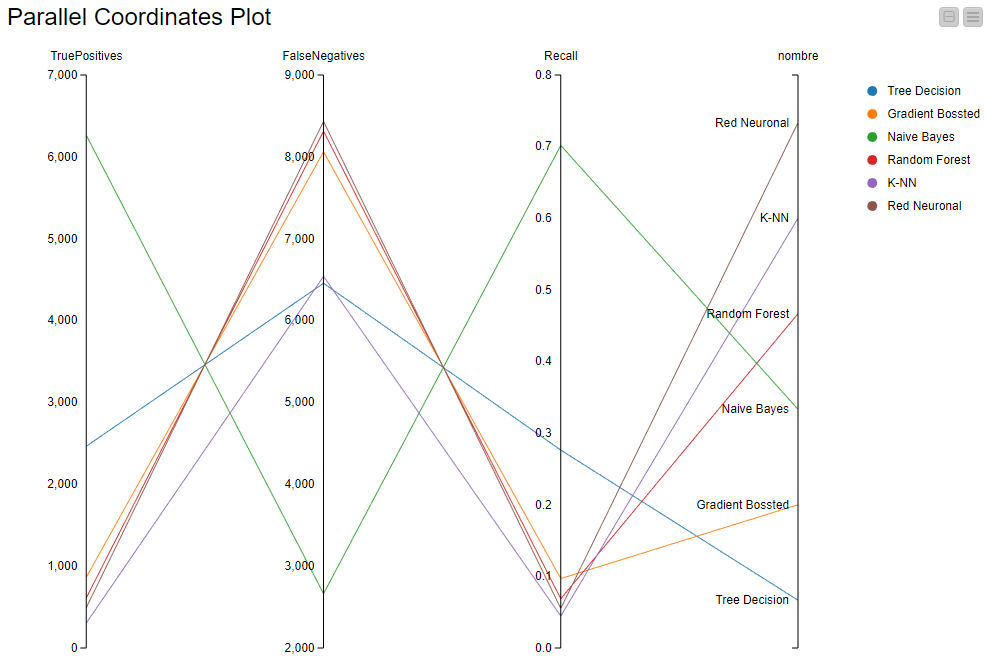
\includegraphics[width=0.9\textwidth]{./imagenes/37}
		\caption{Grafica del Recall de los 6 algoritmos , integrando tanto verdaderos positivos como falsos negativos} \label{fig:1}
	\end{figure}

	En cuanto a los resultados obtenidos de los seis algoritmos respecto al Specifity o TNR se tiene la figura 3.5. En ella se tienen en cuenta las variables
	de falsos positivos y verdaderos negativos, que son las que intervienen en el calculo del Specifity. En esta gráfica se puede apreciar porque unos algoritmos tienen 
	mejor Specifity que otros. En primer lugar se aprecia como Red Neuronal , K-NN  , Random Forest y Gradient Boosted tienen los mejores resultados de Specifity . Al contrario 
	que con el Recall , el algoritmo Naive Bayes se posiciona en último lugar , por lo que tenemos con Naive Bayes un modelo un poco 'indeciso' debido al gran aumento de falsos negativos.
	También merece la pena ver como el algoritmo Red Neuronal esta en primera posición.  \\

	\begin{figure}[htb]
		\centering
		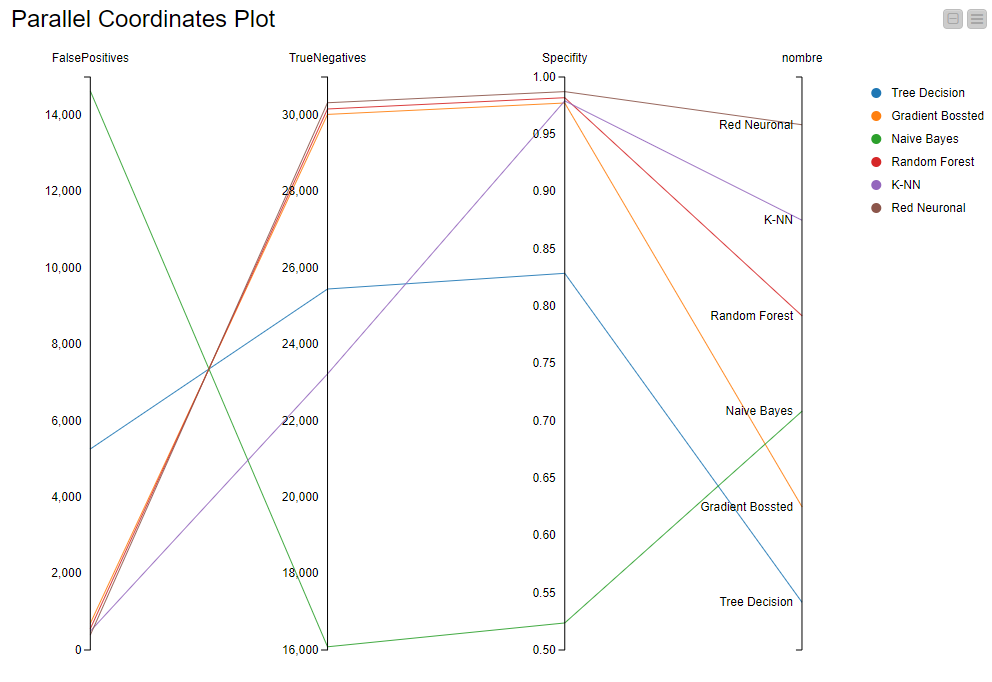
\includegraphics[width=0.9\textwidth]{./imagenes/38}
		\caption{Grafica del Specifity de los 6 algoritmos , integrando tanto falsos positivos como verdaderos negativos} \label{fig:1}
	\end{figure}

	Lo que se puede observar con las gráficas 3.4 y 3.5 es que algoritmos son regulares al Recall y Specifity. Por lo que sus modelos (en su configuración por defecto) 
	se adaptan bien a nuestro tipo concreto de datos. \\

	Para finalizar esta comparativa vamos a ver en la figura 3.6 el comportamiento de los algoritmos en cuanto a su Accuracy se refiere. Se puede apreciar que los 4 algoritmos dominantes
	son GradientBoosted, RandomForest, K-NN Y Red Neuronal. Dejando a NaiveBayes 'por los suelos' .

	\begin{figure}[htb]
		\centering
		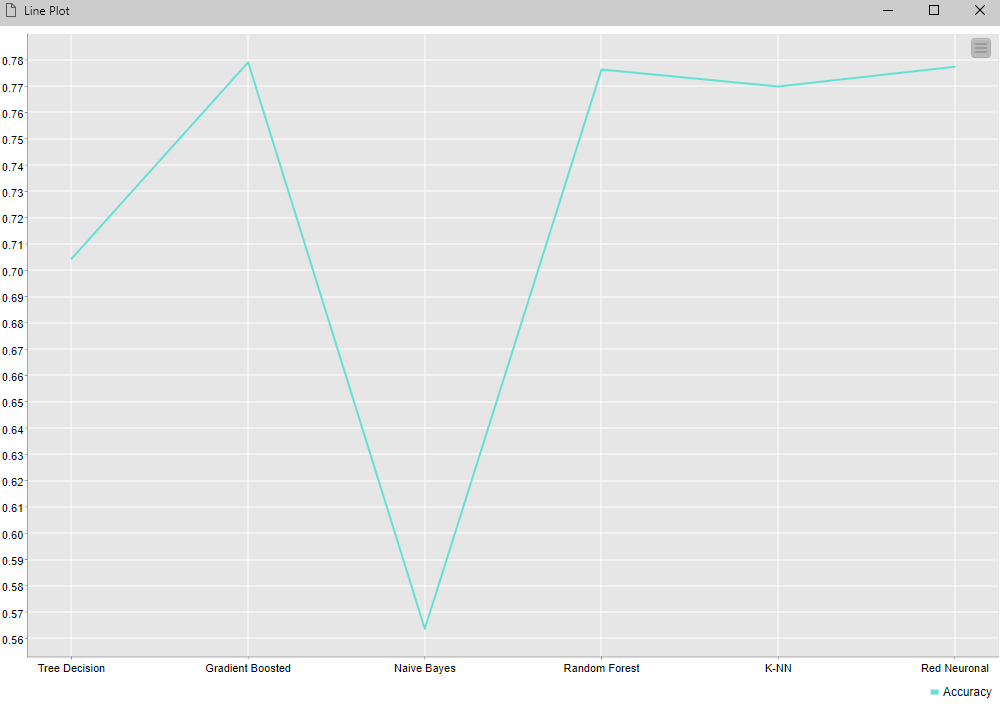
\includegraphics[width=0.8\textwidth]{./imagenes/39}
		\caption{Grafica del Accuracy de los 6 algoritmos} \label{fig:1}
	\end{figure}

	Para finalizar decimos que los algoritmos GradientBoosted , RandomForest y Red Neuronal son los que mejor se están comportando en nuestro estudio con las configuraciones 
	por defecto. 
	
	%-----------------------------------------------------------------------
	%							Configuraci´on de algoritmos
	%----------------------------------------------------------------------	
	\section[Configuración de algoritmos]{Configuración de algoritmos.}
	
	En este apartado vamos a comentar los distintos parámetros y configuraciones usadas a lo largo de la práctica. A su vez se mostrará para algunos algoritmos una configuración diferente y se compararán los resultados, en donde podremos ver aspectos como el sobre aprendizaje y la obtención de modelos más simples
	
	%----------------------------------------------------------------------
	%							Decision Tree
	%----------------------------------------------------------------------
	
	\subsection{Decision Tree}
	
	En primer lugar tenemos el árbol de decisión con sus valores por defecto, en este caso los parámetros de configuración son los del nodo Decision Tree Learner. En la figura 4.1 se puede apreciar la columna de la clase, la cuál será siempre la misma. Como medida de calidad está indicado el Gini Index y no hay método de poda seleccionado.
	En cuanto al mínimo número de registros por nodo viene por defecto en 2. Y el número de registros para almacenar por vista en 10000.	\\
	
	\begin{figure}[htb]
		\centering
		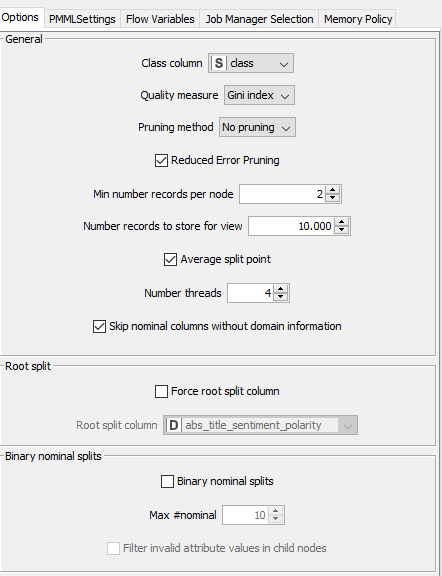
\includegraphics[width=0.4\textwidth]{./imagenes/40}
		\caption{Configuración por defecto del algoritmo Decision Tree} \label{fig:1}
	\end{figure}
	
	Para intentar sacar otro modelo vamos a aumentar el número mínimo de registros por nodo, de 2 a  10. La configuración es la que se muestra en la figura 4.2 .Con esto podemos estar ocasionando pérdida de precisión, pero si ocurre que la pérdida es poca, podríamos estar ante una mejor solución, por la mayor simplicidad del modelo. En cuanto al número de registros para almacenar por vista lo dejaremos en 10000.
	
	\begin{figure}[htb]
		\centering
		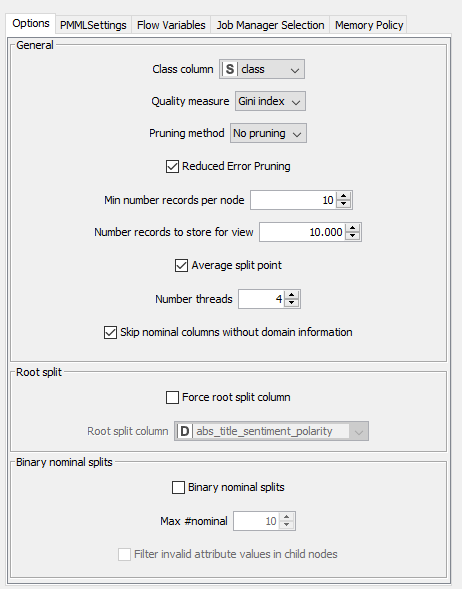
\includegraphics[width=0.4\textwidth]{./imagenes/41}
		\caption{Configuración version 2.0 algoritmo Decision Tree} \label{fig:1}
	\end{figure}
	
	Para comparar los resultados extraemos una tabla con los resultados de ambas configuraciones (figura 4.3) , así como sus gráficas ROC para ver sus curvas (figura 4.4). \\
	
	\begin{figure}[htb]
		\centering
		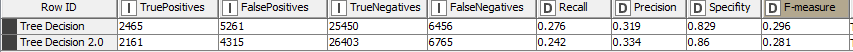
\includegraphics[width=1.0\textwidth]{./imagenes/42}
		\caption{Tabla comparativa de las configuraciondes de Decision Tree} \label{fig:1}
	\end{figure}
	
	\begin{figure}[htb]
		\centering
		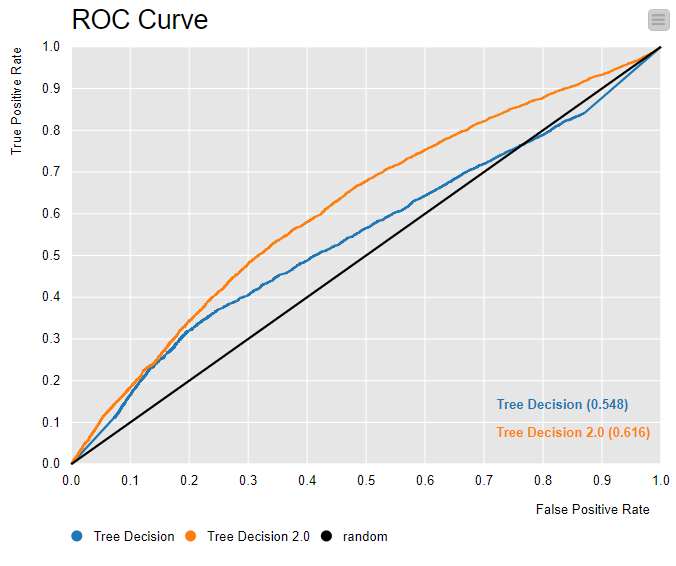
\includegraphics[width=0.8\textwidth]{./imagenes/43}
		\caption{Graficas ROC de las configuraciondes de Decision Tree} \label{fig:1}
	\end{figure}
	
	En este caso se puede ver como el modelo con la configuración por defecto estaba sobre aprendiendo , de forma que se sobre adaptaba a los datos de entrenamiento y con los datos de test no cumplía con las expectativas. La forma mas clara de apreciarlo es que simplificando el modelo se tienen mejores resultados. Por lo que estamos obteniendo un modelo más simplificado y ganando precisión. 
	
	%----------------------------------------------------------------------
	%							Gradient Boosted
	%----------------------------------------------------------------------
	
	\subsection{Gradient Boosted}
	
	Pasando al segundo algoritmo, vamos a ver los parámetros que tiene por defecto. Parámetros como la selección de atributos, numero limite de niveles (profundidad) , numero de modelos o tasa de aprendizaje. La figura 4.5 muestra la configuración por defecto, donde tenemos el límite de profundidad del árbol en 4.
	
	\begin{figure}[htb]
		\centering
		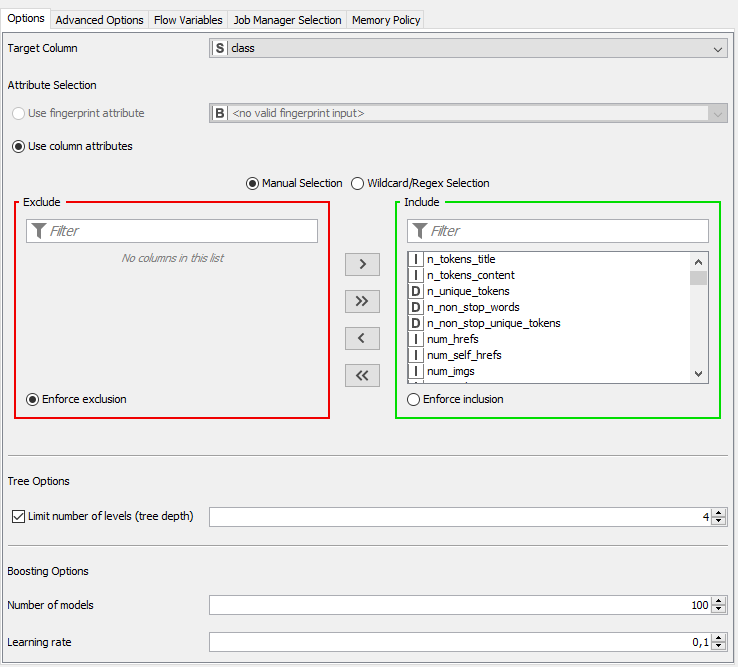
\includegraphics[width=0.8\textwidth]{./imagenes/44}
		\caption{Configuración por defecto del algoritmo Gradient Boosted} \label{fig:1}
	\end{figure}
	
	Para intentar sacar un modelo más preciso y ver las diferencias entre ambos modelos , vamos a aumentar el límite de profundidad del árbol de 4 a 10 , e incrementar el numero de modelos de 100 a 200, como muestra la figura 4.6.
	
	\begin{figure}[htb]
		\centering
		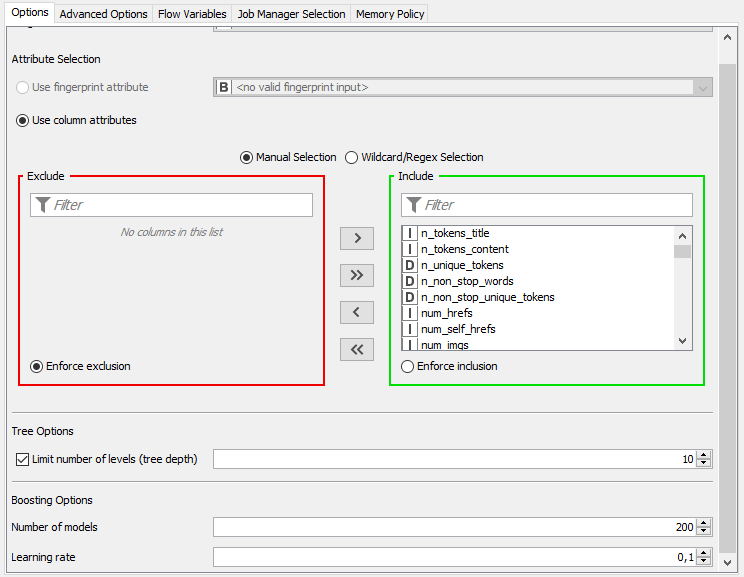
\includegraphics[width=0.8\textwidth]{./imagenes/45}
		\caption{Configuración version 2.0 del algoritmo Gradient Boosted} \label{fig:1}
	\end{figure}
	
	Para comparar los resultados extraemos una tabla con los resultados obtenidos de ambas configuraciones (figura 4.7) , así como sus gráficas ROC para ver sus curvas (figura 4.8). \\
	
	\begin{figure}[htb]
		\centering
		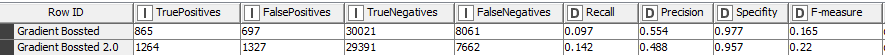
\includegraphics[width=1.0\textwidth]{./imagenes/46}
		\caption{Tabla comparativa de las configuraciondes de Decision Tree} \label{fig:1}
	\end{figure}
	
	\begin{figure}[htb]
		\centering
		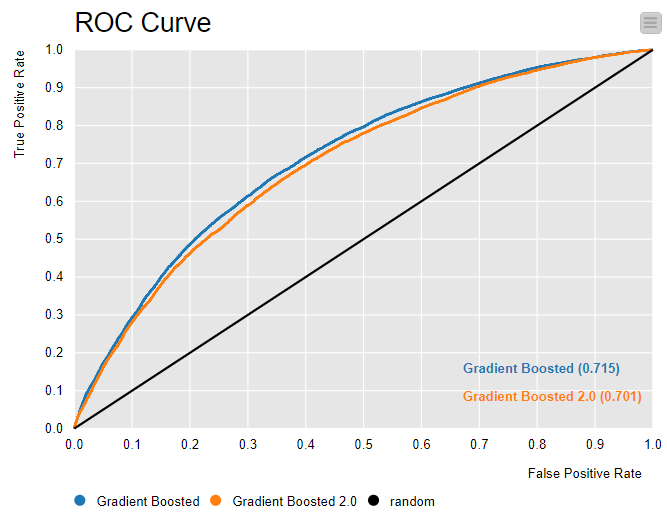
\includegraphics[width=0.8\textwidth]{./imagenes/47}
		\caption{Graficas ROC de las configuraciondes de Decision Tree} \label{fig:1}
	\end{figure}
	
	En este caso , vemos como aumentando la complejidad y el tiempo de ejecución del modelo no conseguimos mejorar sustancialmente los resultados, sino que hemos perdido Precisión y Specifity, provocado por el aumento de falsos positivos.
	
	En contraposición nos encontramos con un Recall en aumento en el segundo algoritmo, ya que se distancia con respecto los otros dos en verdaderos positivos, siendo los falsos negativos prácticamente similares a los demás algoritmos.
	
	Con respecto al valor del AUC, apenas se nota la diferencia entre las curvas .
	
	%-----------------------------------------------------------------------
	%							Naive Bayes
	%----------------------------------------------------------------------
	
	\subsection{Naive Bayes}
	
	Para este algoritmo únicamente se han realizado las ejecuciones con los parámetros por defecto. 
	Los parámetros por defecto son : La columna de clasificacion (class), probabilidad por defecto (0.0) , máximo numero de valores nominales únicos por atributo (100), ignorar valores perdidos y crear un modelo compatible PMML (ambos desmarcados). La figura 4.9 muestra esta configuración.
	
	\begin{figure}[htb]
		\centering
		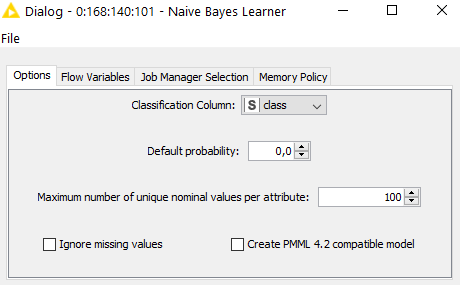
\includegraphics[width=0.5\textwidth]{./imagenes/48}
		\caption{Configuración por defecto del algoritmo Naive Bayes} \label{fig:1}
	\end{figure}
	
	Tanto los resultados como la curva ROC obtenida por este algoritmo se han mostrado con anterioridad en la sección 2.4.
	
	%-----------------------------------------------------------------------
	%							Random Forest
	%----------------------------------------------------------------------
	
	\subsection{Random Forest}
	
	En el caso del algoritmo Random Forest , al igual que en el caso anterior con Naive Bayes, únicamente se han realizado pruebas con los parámetros por defecto. Los parámetros que nos encontramos son los siguientes: Columnas de atributos que añadimos (todos) , patrones a almacenar (2000) , criterio de división (gain ratio) , profundidad del árbol (10), mínimo tamaño del nodo (1), y numero de modelos (100) . La figura 4.10 muestra esta configuración.
	
	\begin{figure}[htb]
		\centering
		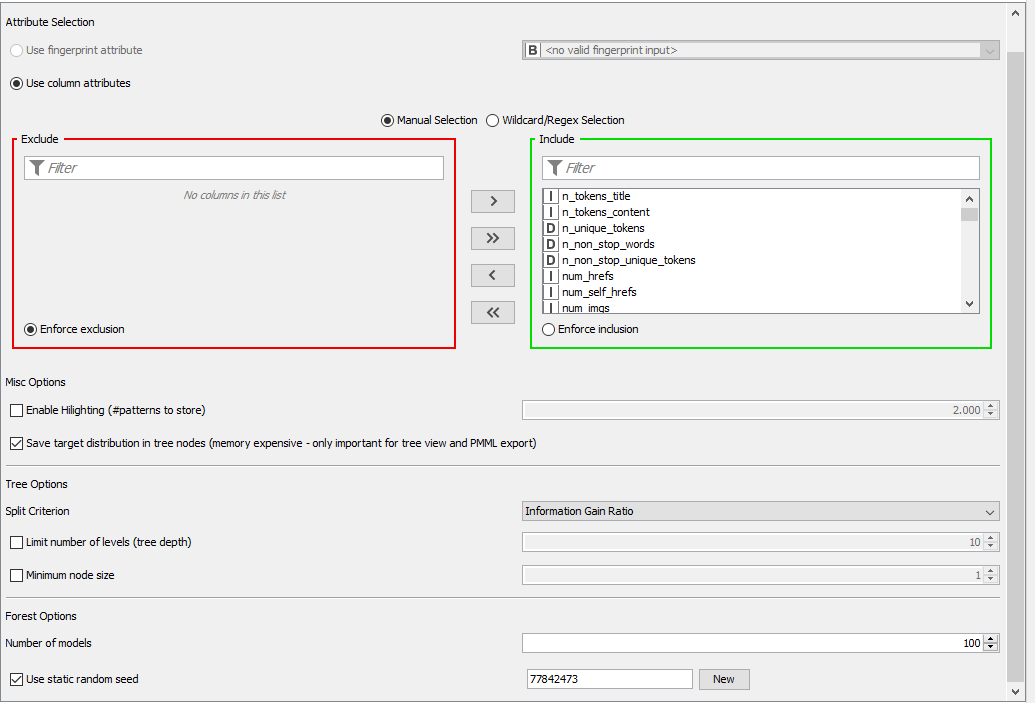
\includegraphics[width=0.8\textwidth]{./imagenes/49}
		\caption{Configuración por defecto del algoritmo Random Forest} \label{fig:1}
	\end{figure}
	
	Tanto los resultados como la curva ROC obtenida por este algoritmo se han mostrado con anterioridad en la sección 2.3.
	
	%-----------------------------------------------------------------------
	%							K-NN
	%----------------------------------------------------------------------
	
	\subsection{K-NN}
	
	Para éste algoritmo se han realizado pruebas con dos configuraciones diferentes.
	
	Una primera configuración con los siguientes parámetros : Columna con la clase (class) , el numero de vecinos a considerar (10) , peso de esos vecinos por distancia (off) y salida de las probabilidades de la clase , que se usa para sacar la gráfica ROC. Esta configuración es la que se representa con la figura 4.11
	
	\begin{figure}[htb]
		\centering
		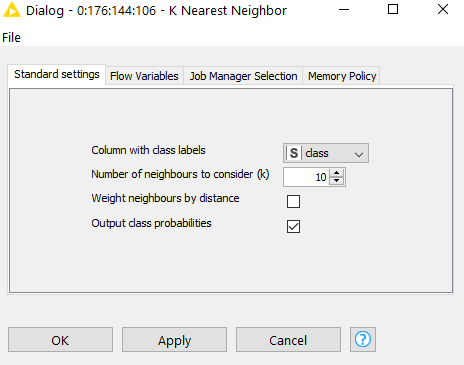
\includegraphics[width=0.5\textwidth]{./imagenes/50}
		\caption{Configuración 1 del algoritmo K-NN} \label{fig:1}
	\end{figure}
	
	La segunda configuración que usamos cuenta con los siguientes parámetros : Columna con la clase (class) , el numero de vecinos a considerar (30) , peso de esos vecinos por distancia (on, incluye la distancia del patrón de consulta a los patrones de entrenamiento , de tal forma que los vecinos mas cercanos tendrán una mayor influencia) y salida de las probabilidades de la clase , que se usa para sacar la gráfica ROC. Esta configuración es la que se representa con la figura 4.12
	
	\begin{figure}[htb]
		\centering
		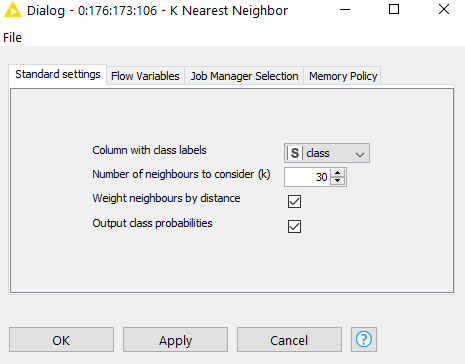
\includegraphics[width=0.5\textwidth]{./imagenes/51}
		\caption{Configuración 2 del algoritmo K-NN} \label{fig:1}
	\end{figure}
		
	Para comparar los resultados , extraemos una tabla con los resultados de ambas configuracienes. (figura 4.13)
	
	\begin{figure}[htb]
		\centering
		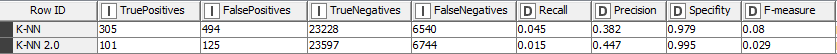
\includegraphics[width=1.0\textwidth]{./imagenes/52}
		\caption{Tabla comparativa de las configuraciondes de K-NN} \label{fig:1}
	\end{figure}
	
	En las dos modificaciones que se han realizado se puede observar que no existe sobre aprendizaje, ya que al aumentar el numero de vecinos y tener en cuenta los pesos , los resultados no mejoran , sino todo lo contrario , empeoran. Disminuye el numero de verdaderos positivos y aumenta el de falsos negativos. Cabe destacar que mejoran la Precision y el Specifity respecto a la primera configuración con 10 vecinos.
	
	%----------------------------------------------------------------------
	%							Red Neuronal
	%----------------------------------------------------------------------
	
	\subsection{Red Neuronal}
	
	Por último, tenemos el algoritmo Red Neuronal en donde se han realizado una comparación como en los casos anteriores, modificando los ajustes y parámetros de configuración propios del algoritmo. \\
	
	En cuanto a la configuración por defecto tenemos, parámetro de máximo numero de iteraciones (100) , numero de capas ocultas (1), numero de neuronas ocultas por capa (10), ignorar valores perdidos (on) y semilla (mi DNI). Configuración que se muestra en la figura 4.14
	
	\begin{figure}[htb]
		\centering
		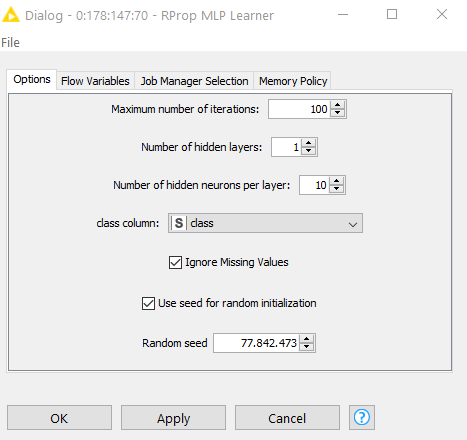
\includegraphics[width=0.5\textwidth]{./imagenes/53}
		\caption{Configuración por defecto del algoritmo Red Neuronal} \label{fig:1}
	\end{figure}
	
	En lo que se refiere al modelo modificado de Red Neuronal , se ha modificado el numero de capas ocultas de 1 a 15, y el numero de neuronas ocultas de cada capa a 20. Esto provoca un modelo mas complejo , que no puede visualizarse y por lo tanto sacar conclusiones claras de el como por ejemplo un árbol de decisión. Esta configuración es la que se muestra en la figura 4.15
	
	\begin{figure}[htb]
		\centering
		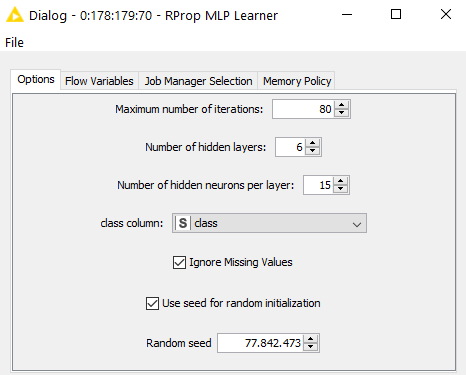
\includegraphics[width=0.5\textwidth]{./imagenes/57}
		\caption{Configuración modificada del algoritmo Red Neuronal} \label{fig:1}
	\end{figure}
	
	Para comparar los resultados extraemos una tabla con los resultados obtenidos de ambas configuraciones (figura 4.16) , así como sus gráficas ROC para ver sus curvas (figura 4.17). \\
	
	\begin{figure}[htb]
		\centering
		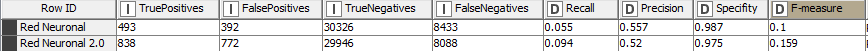
\includegraphics[width=1.0\textwidth]{./imagenes/55}
		\caption{Tabla comparativa de las configuraciondes de Red Neuronal} \label{fig:1}
	\end{figure}
	
	\begin{figure}[htb]
		\centering
		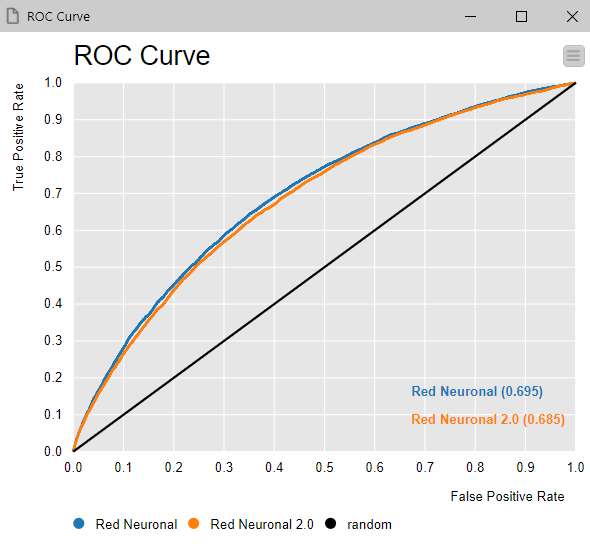
\includegraphics[width=0.8\textwidth]{./imagenes/56}
		\caption{Graficas ROC de las configuraciondes de Red Neuronal} \label{fig:1}
	\end{figure}
	
	En los resultados obtenidos se puede apreciar la existencia de sobre aprendizaje , ya que en el primer caso con la configuración se obtienen mejores resultados que con un modelo mas complejo con mayor numero de capas  ocultas y de neuronas por capa. El modelo por defecto tiene mejor Precision , Specifity , y AUC (esta última se puede apreciar en la gráfica ROC). \\
	
	Este estudio de los resultados realizado se ve afectado por el pre procesamiento aleatorio de los datos. Procesamiento que se explico en secciones anteriores y que se modificara en distintas versiones posteriormente.

	%-----------------------------------------------------------------------
	%							Procesado de datos
	%----------------------------------------------------------------------	
	\section[Procesado de datos]{Procesado de datos.}	
	
	En esta sección se habla de los distintos pre-procesados de datos que se han realizado para algunos de los algoritmos con la intención de mejorar los resultados que hemos obtenido hasta ahora, aunque en algunos casos no conseguimos nuestro objetivo de mejorar el modelo. Aun así es interesante conocer los distintos comportamientos de los algoritmos. Las funcionalidades de los nodos usados para el procesado de datos en KNIME han sido normalizar, filtrar, discretizar , etc... \\
	
	Para nuestro caso nos hemos centrado en los algoritmos de Decision Tree, Naive Bayes y Random Forest. Estos dos últimos han sido elegidos por el hecho de que en la sección anterior no se realizo un estudio de las diferentes configuraciones posibles. 
	
	%----------------------------------------------------------------------
	%							Decision Tree
	%----------------------------------------------------------------------
	
	\subsection{Decision Tree}
	
	Para este algoritmo hemos considerado las dos versiones obtenidas del apartado 4.1 y le hemos aplicado el siguiente procesamiento:\\
	
	One to Many: Transforma todos los posibles valores de una columna en una nueva columna. De tal forma que en las nuevas columnas sale 1 cuando la fila pertenece a ese valor, y 0 cuando no. El nodo agrega tantas columnas como posibles valores . En nuestro caso lo hacemos con la columna de weekday (String). \\
	
	Column filter: Elimina las columnas que previamente han sido transformadas en nuevas columnas por el nodo One to Many. En nuestro caso eliminamos la columna weekday (String) \\
	
	Missing Values: Maneja los valores perdidos de las distintas celdas, de tal forma que se puede actuar reponiendo valores en forma de media , mas frecuente o eliminar la fila. Para nuestro caso lo usaremos para las casillas numéricas , sustituyendo el valor perdido por la media, y para las string pondremos el valor mas frecuente. \\
	
	Normalizer: Normaliza los valores de las columnas numéricas entre el rango que se desee. Para nuestro caso entre 0 y 1.\\
	
	A continuacion se muestra la figura 5.1 con el Workflow usado en KNIME para el procesamiento de los datos. 
	
	\begin{figure}[htb]
		\centering
		\includegraphics[width=0.8\textwidth]{./imagenes/58}
		\caption{Workflow en Knime para el procesado de Decision Tree} \label{fig:1}
	\end{figure}
	
	Para comparar los resultados obtenidos sin y con el procesado se muestra la figura 5.2 como tabla comparativa. Así como la figura 5.3 con las curvas ROC de los resultados obtenidos sin y con el procesado de datos.
	
	\begin{figure}[htb]
		\centering
		\includegraphics[width=1.0\textwidth]{./imagenes/59}
		\caption{Comparativa de Resultados de Decision Tree, sin y con procesado} \label{fig:1}
	\end{figure}
	
	\begin{figure}[htb]
		\centering
		\includegraphics[width=0.8\textwidth]{./imagenes/60}
		\caption{Comparativa de curva ROC de Decision Tree, sin y con procesado} \label{fig:1}
	\end{figure}
	
	Con este procesamiento se ha conseguido que el algoritmo trabaje sin columnas categóricas, eliminando las mismas y convirtiéndolas en nuevas columnas numéricas , sin valores perdidos y normalizando el conjunto de valores a una escala apropiada. A través de la comparativa de resultados y de las graficas ROC se puede deducir que con el procesado se consigue un mejor Recall , peor Precision y peor Specfifity. Respecto al AUC de cada par de algoritmos con y sin procesado no se aprecian diferencias significativas.
	
	%----------------------------------------------------------------------
	%							Random Forest
	%----------------------------------------------------------------------
	
	\subsection{Random Forest}
	
	Para el algoritmo Random Forest hemos considerado 2 preprocesamientos diferentes: \\
	
	El primero es el mismo procesamiento que el utilizado en el apartado anterior con el algoritmo Decision Tree. Los nodos usados son One to Many, Column Filter, Missing Values y Normalicer, todos ellos con la misma configuracion . La figura 5.1 muestra el Workflow usado en KNIME para primer procesamiento de los datos. \\
	
	A continuacion se muestra la figura 5.4 con el Workflow usado en KNIME para el segundo procesamiento de los datos, en el hemos usado los siguientes nodos: \\
	
	\begin{figure}[htb]
		\centering
		\includegraphics[width=0.8\textwidth]{./imagenes/61}
		\caption{Workflow en Knime para el procesado 2 de Random Forest} \label{fig:1}
	\end{figure}
	
	Equal Size Sampling: Elimina filas aleatoriamente pertenecientes a la clase de la mayoria, de tal forma que devuelve todas las filas de la clase minoritaria y una muestra aleatoria de la clase mayoritaria, realizando un balanceo entre clases. (UnderSampling). \\
	
	Missing Values: Maneja los valores perdidos de las distintas celdas, de forma que se puede actuar reponiendo valores de distintas formas. En nuestro caso lo usamos para sustituir los valores numericos perdidos por la media.\\
	
	Normalizer: Normaliza los valores de las columnas numéricas en el rango deseado , en nuestro caso usamos el rango entre 0 y 1 para todos los valores numericos \\
	
	Para comparar los resultados obtenidos sin y con el procesado se muestra la figura 5.5 como tabla comparativa. Así como la figura 5.6 con las curvas ROC de los resultados obtenidos sin y con el procesado de datos.
	
	\begin{figure}[htb]
		\centering
		\includegraphics[width=1.0\textwidth]{./imagenes/62}
		\caption{Comparativa de Resultados de Random Forest, sin y con procesado} \label{fig:1}
	\end{figure}
	
	\begin{figure}[htb]
		\centering
		\includegraphics[width=0.8\textwidth]{./imagenes/63}
		\caption{Comparativa de curva ROC de Random Forest, sin y con procesado} \label{fig:1}
	\end{figure}
	
	Con este procesamiento se ha conseguido que el algoritmo trabaje sin columnas categóricas, eliminando las mismas y convirtiéndolas en nuevas columnas numéricas , sin valores perdidos y normalizando el conjunto de valores a una escala apropiada. A través de la comparativa de resultados y de las graficas ROC se puede deducir que con el procesado se consigue un mejor Recall , mejor Precision y peor Specfifity en el caso del preprocesado 2. Respecto al AUC de los algoritmos con y sin procesado no se aprecian diferencias.
	
	%----------------------------------------------------------------------
	%							Naive Bayes
	%----------------------------------------------------------------------
	
	\subsection{Naive Bayes}
	
	Para este algoritmo hemos considerado 2 preprocesamientos diferentes.\\
	
	En primer lugar hemos usado el procesamiento común a los dos algoritmos anteriores (figura 5.1) y en segundo lugar hemos usado el procesamiento de la subseccion anterior (figura 5.4). \\
	
	Para comparar los resultados obtenidos sin y con el procesado se muestra la figura 5.7 como tabla comparativa. Así como la figura 5.8 con las curvas ROC de los resultados obtenidos sin y con el procesado de datos.
	
	\begin{figure}[htb]
		\centering
		\includegraphics[width=1.0\textwidth]{./imagenes/64}
		\caption{Comparativa de Resultados de Naive Bayes, sin y con procesado} \label{fig:1}
	\end{figure}
	
	\begin{figure}[htb]
		\centering
		\includegraphics[width=0.8\textwidth]{./imagenes/65}
		\caption{Comparativa de curva ROC de Naive Bayes, sin y con procesado} \label{fig:1}
	\end{figure}
	
	Con este procesamiento se ha conseguido que el algoritmo trabaje sin columnas categóricas, eliminando las mismas y convirtiéndolas en nuevas columnas numéricas , sin valores perdidos y normalizando el conjunto de valores a una escala apropiada. A través de la comparativa de resultados y de las gráficas ROC se puede deducir que con el procesado se consigue un mejor Recall , mejor Precision y peor Specfifity. Respecto al AUC de los algoritmos con y sin procesado no se aprecian diferencias (se observa en la grafica ROC).
	
	%-----------------------------------------------------------------------
	%							Interpretación de resultados
	%----------------------------------------------------------------------	
	\section[Interpretación de resultados]{Interpretación de resultados.} 
	
	%-----------------------------------------------------------------------
	%							Bibliografía
	%----------------------------------------------------------------------	
	\section[Bibliografía]{Bibliografía.}

	
	%-----------------------------------------------------------------------
	%							BIBLIOGRAFIA
	%-----------------------------------------------------------------------
	% Referencia a bibliografia			En \cite{Baz}
	% Referencia a figura				La figura (\ref{fig:1})
	% Espacio entre lineas				\vspace{0.06in} o \\
	% Figura con comentario al pie
	%\begin{figure}[htb]
	%	\centering
	%	\includegraphics[width=0.4\textwidth]{./imagenes/1}
	%	\caption{Universidad de Granada.} \label{fig:1}
	%\end{figure}

	\begin{thebibliography}{99}
		\bibitem{Wikipedia1} 
		\textsc{Clasificador bayesiano}
		%\textit{Programacuib}.
		\newline
		\url{https://es.wikipedia.org/wiki/Clasificador_bayesiano_ingenuo}
		\bibitem{Wiki1} 
		\textsc{Clasificador de bayes}
		\newline
		\url{https://nlp.stanford.edu/IR-book/html/htmledition/naive-bayes-text-classification-1.html}
		\bibitem{sci2s.ugr.es} 
		\textsc{onlinespopularity}
		\newline
		\url{https://sci2s.ugr.es/sites/default/files/files/Teaching/GraduatesCourses/InteligenciaDeNegocio/Curso18-19/onlinenewspopularity.xlsx}	
		\bibitem{Wikipedia2} 
		\textsc{Decision Tree}
		\newline
		\url{https://es.wikipedia.org/wiki/%C3%81rbol_de_decisi%C3%B3n}	
		\bibitem{Wiki2} 
		\textsc{Decision Tree}
		\newline
		\url{https://www.gestiondeoperaciones.net/procesos/arbol-de-decision/}	
		\bibitem{Wikipedia3} 
		\textsc{Gradient boosting}
		\newline
		\url{https://en.wikipedia.org/wiki/Gradient_boosting}
		\bibitem{Wiki3} 
		\textsc{Gradient boosting}
		\newline
		\url{https://statweb.stanford.edu/~jhf/ftp/trebst.pdf}
		\bibitem{Wikipedia4} 
		\textsc{Random forest}
		\newline
		\url{https://es.wikipedia.org/wiki/Random_forest}
		\bibitem{Wikipedia5} 
		\textsc{K-NN}
		\newline
		\url{https://es.wikipedia.org/wiki/K_vecinos_m%C3%A1s_pr%C3%B3ximos}
		\bibitem{Wikipedia6} 
		\textsc{Red Neuronal}
		\newline
		\url{https://es.wikipedia.org/wiki/Red_neuronal_artificial}
	\end{thebibliography}

	


\end{document}